\part{神经系统疾病}
\markboth{总论}{总论}

\begin{figure}[htbp]
	\centering
	\includegraphics[width=1.0\linewidth]{chap57/fig_57_0}
	\caption{\textit{梵高}在\textit{阿尔勒}的卧室。
		梵高写信给他的朋友兼画家\textit{高更},他感觉到的“我的视力异常疲惫。
		好吧,我休息了两天半,然后又回去工作。
		但我还不敢出去,我做了……卧室的30号帆布,上面有你知道的白木家具。
		啊,好吧,做这个裸露的室内设计让我非常开心。
		很简单。
		色调平淡,但粗糙地刷上了完整厚涂的颜料,墙壁淡紫色,地板椅子和床是铬黄色的,枕头和床单是浅柠檬绿色的,毯子是血红色的,梳妆台是橙色的,脸盆是蓝色的,窗户是绿色的。
		我本想用所有这些非常不同的音调来表达完全的休息,你看,其中唯一的白色是镜子用黑色框架发出的小音符(也用来填充第四对补语)。”
		梵高曾有过精神病发作,但在所考虑的理论中,关于其原因仍存在争议,这些理论包括躁郁症、颞叶癫痫、梅毒、精神分裂症,甚至是毛地黄植物(当时治疗精神疾病的药物)的毒性,以及他油画中的铅中毒和苦艾酒的消耗(阿姆斯特丹的梵高博物馆)。}
	\label{fig:59_0}
\end{figure}


他记得,在癫痫发作期间,或者更确切地说,在癫痫发作之前,他总是经历过一两个时刻,他的整个心脏、大脑和身体似乎都在活力和光明中醒来;
当他充满喜悦和希望,所有的焦虑似乎都被永远扫除;
这些时刻只是预感,因为这是他突然发作的最后一秒(从未超过一秒)。
当然,那一秒是无法形容的。
当他的袭击结束,王子反思自己的症状时,他常对自己说:“虽然这些时间很短,但我对自己的极端意识以及因此比其他时候更多的生命都是由于疾病导致的正常状况的突然破裂。
因此,它们实际上不是一种更高的生活,而是一种更低的生活。”
然而,这种推理,似乎以矛盾告终,并导致进一步的思考:
“尽管这只是疾病,大脑的异常紧张,但如果当我回忆和分析这一时刻时,它似乎是最高程度的和谐与美,那又有什么关系呢?
那是最深刻感觉的瞬间,充满了无限的喜悦和狂喜、热情的奉献、以及最完整的生活?”
尽管听起来很模糊,\textit{梅希金}完全可以理解,尽管他知道这只是他感觉的微弱表达。


大脑和大脑之间关系的本质究竟是什么?
\textit{陀思妥耶夫斯基}自己的癫痫经历深刻地影响了他的写作,在这篇文章中,他探讨了一些关于人类经验的最深刻问题。
我们的思想和情绪仅仅是化学物质和电信号的短暂组合吗?
我们对他们有什么影响吗?
如果没有,我们能为自己的行为负责吗?
如果我们的一些高峰经历只是愉快的化学事故呢?
或者,正如\textit{缪什金王子}(陀思妥耶夫斯基小说《白痴》的主角)所想的那样,如果我们的一些巅峰状态是疾病带来的幸福事故呢?那么,“变得更好”意味着什么?
例如,患有躁郁症的人可能很难放弃伴随躁狂症的广阔情感和创造力。


尽管这些深刻的问题是哲学家而不是神经科学家的权限,但很少有情况会像成为神经疾病或精神疾病的受害者那样,对大脑与大脑的关系产生如此尖锐的质疑。
这些疾病的范围很广,从运动障碍到癫痫,精神分裂症,情绪失衡,认知障碍,神经退行性疾病,甚至衰老。
我们了解得越多,就越明显,这些疾病产生了非常广泛的影响,模糊了它们之间的分类界限。
例如,帕金森病等所谓的运动障碍涉及认知变化和情感变化;
诸如孤独症或精神分裂症等认知障碍可能有非常明显的身体表现。


尽管这些界限有些模糊,但本节的每一章都将从神经科学的角度研究每种主要疾病的基本原理。
就目前所知,这里的重点是分子机制。
也许令人惊讶的是,如此多不同的疾病似乎集中在一个生理点上:突触功能。
在孤独症和几种精神疾病中,突触发育异常;
在癫痫中,异常的离子通道活动会干扰兴奋性和抑制性神经元突触输入的平衡。
衰老和神经退行性疾病通过蛋白质和\textit{核糖核酸}稳态的逐渐改变而导致突触丧失,这会损害正常的细胞功能。


这种观察有助于塑造你即将遇到的材料,但不应用于过于简化。
任何受到还原论诱惑的人都会很好地参与陀思妥耶夫斯基和梵高等伟大艺术家的作品,他们代表了人类经历的所有痛苦和荣耀的复杂性。




\chapter{周围神经和运动单元疾病} \label{chap:chap57}

大脑处理复杂信息的一项主要任务是处理骨骼肌的收缩,其决定何时以及如何移动在很大程度上是由神经系统的进化作为驱动(第~\ref{chap:chap30}~章)。


除了最原始的动物外,所有动物的运动都是由特定的肌肉细胞控制。
肌肉一般分为以下 3 种类型:
平滑肌主要用于内部活动,例如蠕动和控制血液流动;
心肌主要用于心脏泵血;
骨骼肌主要用于骨骼运动。
在本章中,我们将研究哺乳动物的各种神经系统疾病,这些疾病通过改变运动神经的动作电位传导、从神经到肌肉的突触传递和肌肉收缩来影响运动。


1925年,\textit{查尔斯$\cdot$谢林顿}引入了术语“运动单元”,用来表示运动功能的基本单元,包括一个运动神经元及其支配的一组肌纤维群(第~\ref{chap:chap31}~章)。
由单个运动神经元支配的肌纤维数量在身体各个部位变化很大,这取决于其所控制运动的灵活性和要移动的身体部位的质量。
因此,不超过100 根肌纤维的运动单元精确控制眼球运动,然而在腿部,单个运动单元多达 1 千根肌纤维。
在特定情况下,一个运动单元支配的所有肌肉都属于同一类型。
此外,无论是自主的还是反射性的运动,运动单元都以固定顺序来进行募集。
最小的运动单元最先被募集,随着肌肉力量的增强,较大的运动单元随后加入。


运动单元是疾病的常见靶标。
运动单元病变的特征因受影响的运动单元功能而异:
(1)运动神经元或感觉神经元的细胞体,
(2)相应的轴突,
(3)神经肌肉接头(运动轴突和肌肉之间的突触),
(4)运动神经元支配的肌纤维。
因此,如图~\ref{fig:57_1}~所示,运动单元疾病通常被分为运动神经元疾病、\textit{周围神经病变}、神经肌肉接头疾病和原发性肌肉疾病(肌病)。


\begin{figure}[htbp]
	\centering
	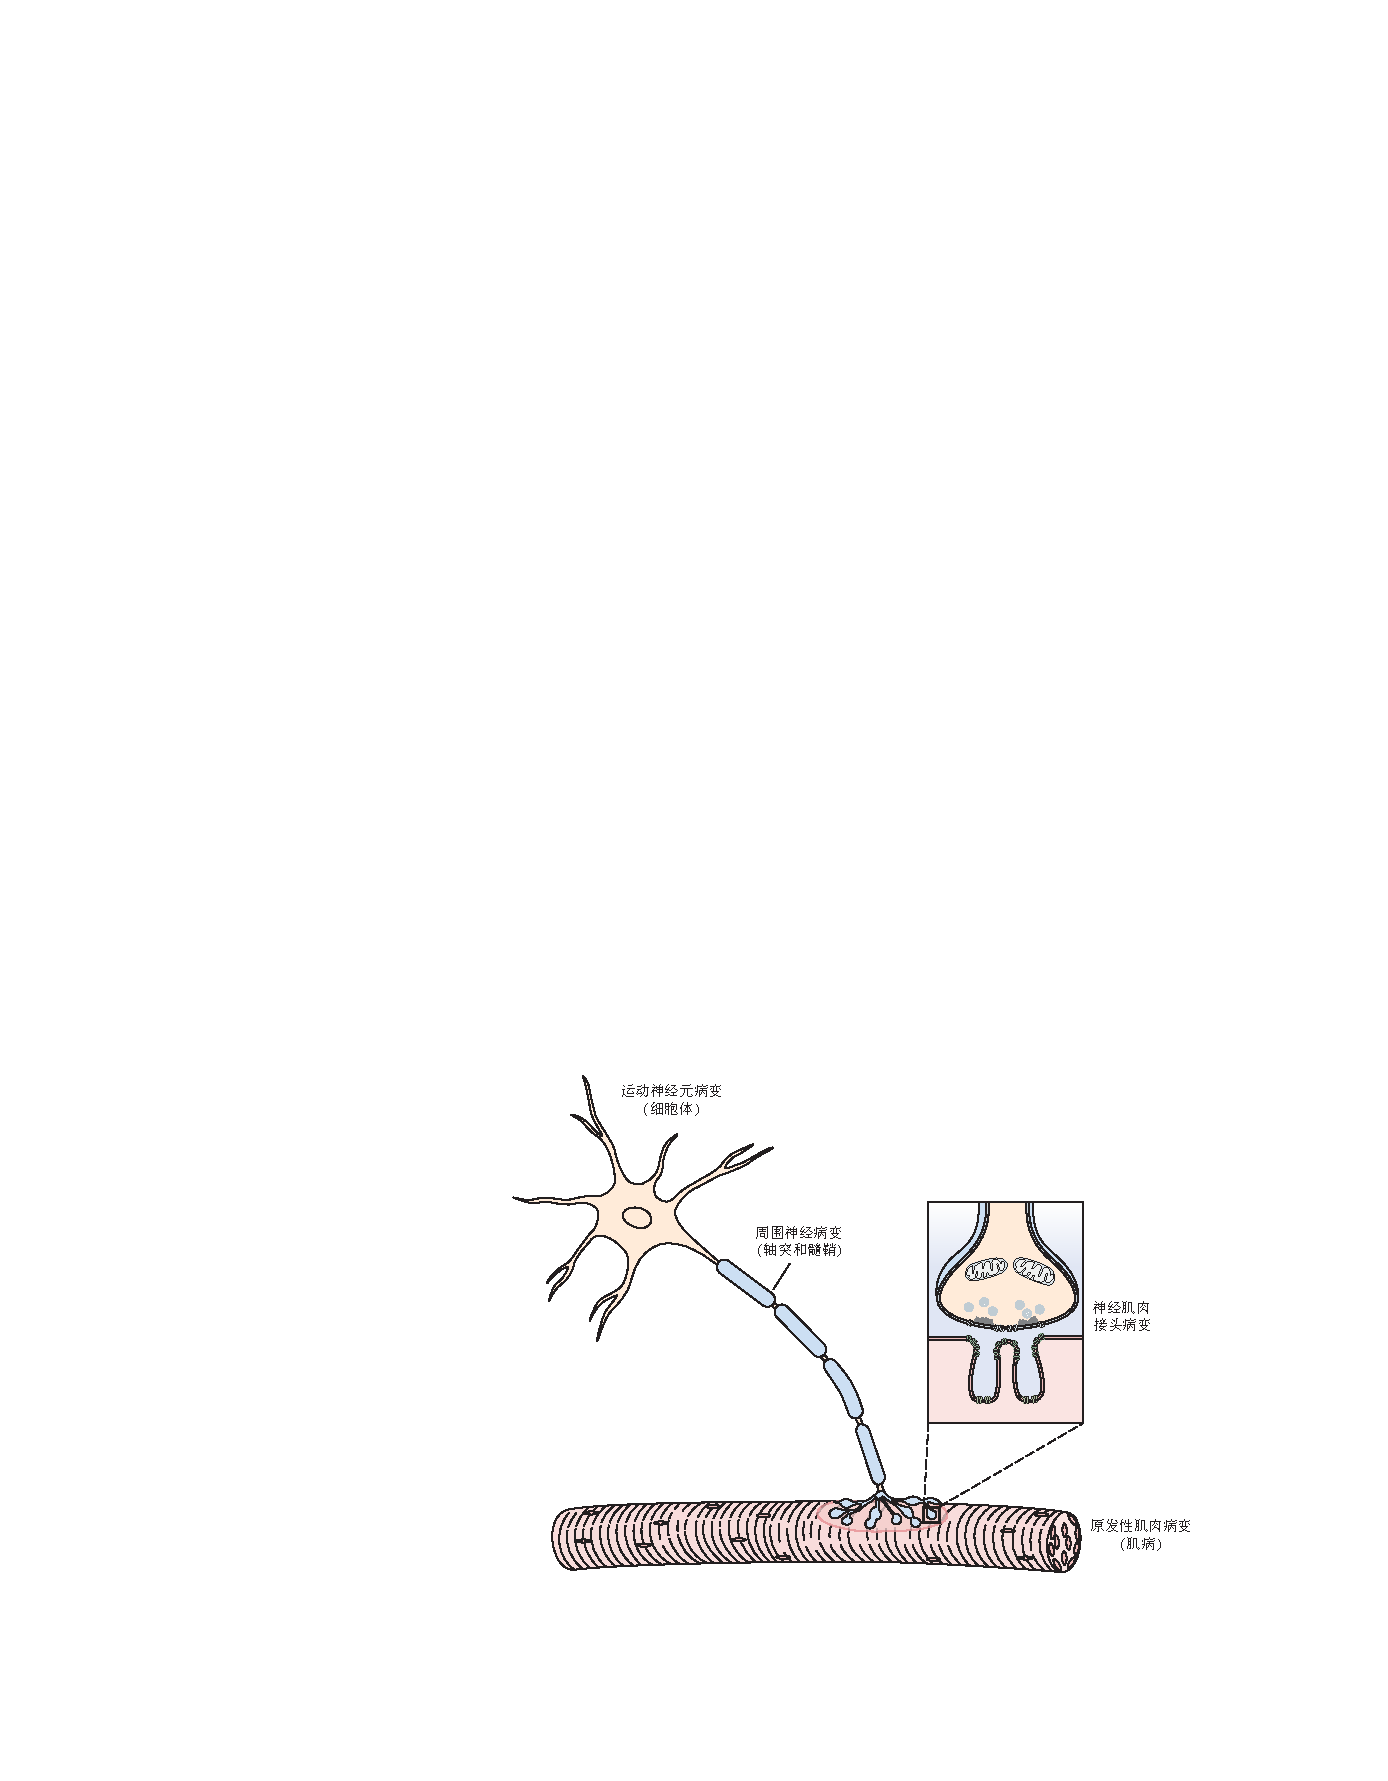
\includegraphics[width=0.91\linewidth]{chap57/fig_57_1}
	\caption{运动单元疾病根据受影响的运动单元部位分成 4 种类型:
		运动神经元病变影响神经元的细胞体、\textit{周围神经病变}则影响轴突、神经肌肉接头病变影响突触的功能、肌病影响肌肉纤维。}
	\label{fig:57_1}
\end{figure}


周围\textit{神经病变}患者会出现运动神经元或其轴突功能异常引起的虚弱,同时由于大多数周围\textit{神经病变}也影响感觉神经元,因此患者可能还会出现感觉问题。
相对地,在运动神经元疾病中,脊髓中的运动神经元和运动束会发生退化,但感觉神经不会受到影响。
但是在肌病中,患者的无力主要是由于肌肉退化,而运动神经元在这个过程中几乎没有或完全没有发生变化。
在神经肌肉接头疾病中,神经肌肉突触的变化会导致间歇性无力。
临床研究和实验室研究通常将周围神经疾病与神经肌肉接头和肌肉疾病区分开来(表~\ref{tab:57_1})。



\begin{table}[htbp]
	\caption{运动单元疾病的鉴别诊断} \label{tab:57_1} \centering
	\begin{tabular}{llll}
		\toprule
		发现 & 神经 & 神经肌肉接头 & 肌肉\\
		\midrule
		\textbf{临床} &  &  &  \\
		虚弱 & ++ & + & ++ \\
		消瘦 & ++ & − & + \\
		肌束震颤 & + & − & - \\
		抽筋 & + & − & +/- \\
		感觉缺失 & +/- & − & - \\
		反射亢进、巴彬斯基征 & +(肌萎缩性侧索硬化) & − & - \\
		\textbf{实验室} &  &  &  \\
		血清肌酸磷酸激酶升高 & - & - & ++ \\
		脑脊液蛋白升高 & +/- & - & - \\
		神经传导减慢 & + & - & - \\
		重复刺激的反应 & 正常 & 减少(重症肌无力) & 正常 \\
		 &  & 增加(\textit{肌无力综合症}) &  \\
		\textbf{肌电图} &  &  &  \\
		\textit{纤维震颤}、束状 & ++ & - & +/- \\
		电位持续时间 & 增加 & 正常 & 减少 \\
		电位振幅 & 增加 & 正常 & 减少 \\
		\textbf{肌肉活检} &  &  &  \\
		孤立性纤维萎缩 & ++ & 正常 & +/- \\
		成组纤维萎缩 & ++ & 正常 & 正常 \\
		肌肉坏死 & 正常 & 正常 & ++ \\
		\bottomrule
	\end{tabular}
\end{table}



\section{周围神经疾病、神经肌肉接头疾病、肌肉疾病可以在临床上加以鉴别}

当周围神经被切断时,受该神经支配的肌肉会立即瘫痪,随后逐渐萎缩。
由于神经携带感觉和运动纤维,因此神经支配的区域会丧失感觉,腱反射也会立即消失。
萎缩该术语(字面意思是缺乏营养)是指原本正常的肌肉逐渐消瘦的过程;
由于历史上的沿用,该术语现在仍出现在几种神经源性的疾病名称中。


肌病是以骨骼肌无力为主要症状的疾病,通常表现为行走困难和举重困难。
除此之外,肌病还伴有其他罕见的症状,包括肌肉无法放松(肌强直)、痉挛、疼痛(肌痛)以及尿液中出现使肌肉呈红色的含血红素蛋白(肌红蛋白尿)。
肌营养不良症是一种具有特殊症状的肌病:
该病具有遗传性,所有症状都是由肌无力引起的,这种无力症状随时间逐渐加重,在组织学上可以观察到肌肉的退变和再生迹象。


神经源性和肌病都以肌肉无力为共同特征,因此区分两者可能比较困难。
初步估计,远端肢体无力通常表现为神经源性疾病,而近端肢体无力表现为肌病。
表~\ref{tab:57_1}~列出了用于鉴别诊断运动单元疾病的主要临床特征和实验室特征。


一项来区分两者非常有用的测试是\textit{肌电图},这是一种临床程序,通过将一根小针插入肌肉,来记录几个相邻运动单元在细胞外的电活动。
3 个很重要的具体测试:静止时的自发活动、自主控制下的运动单元数量、以及每个运动单元动作电位的持续时间和幅度(已经确定了运动单元电位的振幅和持续时间的正常参考值范围;振幅由运动单元内的肌纤维数量决定)。


在正常肌肉中,静息时肌肉的终板外通常没有活动。
当肌肉进行微弱的自主收缩时,随着不同的运动单元的募集,可以记录到一系列运动单元电位。
如图~\ref{fig:57_2}A~所示,而在完全活跃的正常肌肉中,众多的电位以干扰模式重叠,导致无法识别单个电位。


\begin{figure}[htbp]
	\centering
	\includegraphics[width=1.0\linewidth]{chap57/fig_57_2}
	\caption{骨骼肌的电记录揭示了\textit{神经病变}和原发性肌肉疾病的不同特征。
		A. 正常肌肉的典型活动。
		由单个运动神经元支配的肌纤维通常彼此不相邻。
		插入肌肉的针状电极在记录运动单元电位时,由于神经肌肉接头处的高效传输,确保同一神经元支配的每条肌纤维都能产生动作电位并响应运动中的动作电位而收缩。
		在静息状态下的正常肌肉,\textit{肌电图}中不会记录到肌肉的电活动。
		轻微的\textit{自主运动}激活肌肉,会显示出肌肉中特有的细胞外电反应(\textit{运动单元电位波})。
		最大程度的肌肉收缩会从肌肉中产生特征性的复杂电活动爆发(干扰模式)。
		B. 当运动神经元发生病变时,受自主控制的运动单元数量会减少。
		退化的运动神经元(细胞 A)所支配的肌肉纤维因失神经支配而变得萎缩。
		尽管如此,幸存的神经元(细胞 B)会长出轴突分支,重新支配一部分原本失神经的肌肉纤维。
		幸存的运动神经元的轴突即使在静止状态下也会自发放电,从而引起肌束震颤,这是运动神经元疾病的另一个特征。
		单根的失神经纤维也会自发放电,引起\textit{纤维震颤}(顶部轨迹)。
		随着运动神经元 A 的神经输入丢失和运动神经元 B 对去神经纤维的再支配,运动神经元 B 激活时所产生\textit{运动单元电位波}会扩大。
		在这种情况下,肌电图的干涉图样会变得简化。
		C. 当肌肉病变(肌病)时,每个运动单元所包含的肌纤维数量会减少。
		一些肌肉纤维收缩由于受到 2 个运动神经元的支配而变得功能异常。
		在肌电图中,运动单元电位的数量不会减少,甚至比正常情况更少,持续时间会更长,并且是多相的。
		受影响的单个肌纤维有时会自发地收缩,产生\textit{纤维震颤}。
		当肌肉被轻度激活时,\textit{运动单元电位波}的振幅减小。
		最大肌肉收缩后,干涉图案也会显示出振幅减小。}
	\label{fig:57_2}
\end{figure}


在神经源性疾病中,部分失去神经支配的肌肉会在休息状态下出现自发活动。
肌肉可能仍然能够响应自主运动的指令进行收缩,但由于部分运动轴突的丧失,自主控制下的运动单元数量比正常情况少。
如图~\ref{fig:57_2}B~所示,在最大收缩时,运动单元的减少在\textit{肌电图}中表示得非常明显,此时显示的是离散运动单元电位的模式,而不是正常肌肉所呈现的大量干扰模式。
在最近失去神经支配的肌肉中,肌电图还可能记录到自发的低振幅电位,这与单根肌纤维的放电相对应,称为\textit{纤维震颤}电位。
随着神经源性疾病的进展,单个运动单元电位的振幅和持续时间可能会增加,这是因为剩余的轴突生出小分支,这些小分支支配那些因其他轴突丧失而失去神经支配的肌纤维。
因此,幸存下来的运动单元所包含的肌纤维数量多于正常情况。


在肌病中,静止的肌肉没有活动,并且在收缩时运动单元的数量也没有变化。
如图~\ref{fig:57_2}C~所示,但由于每个运动单元中存活的肌纤维较少,导致运动单元电位持续时间更长且更复杂,具有交替的 +/- 极性(多相),并且振幅更小。


如图~\ref{fig:57_3}~所示,外周运动轴突的传导速度也可以通过电刺激和记录的方法来测量。
在脱髓鞘\textit{神经病变}中,运动轴突的传导速度会减慢,但在没有脱髓鞘的\textit{神经病变}(轴突\textit{神经病变})中,传导速度是正常的。


\begin{figure}[htbp]
	\centering
	\includegraphics[width=1.0\linewidth]{chap57/fig_57_3}
	\caption{运动神经传导的速度可以通过记录\textit{复合肌肉动作电位}来确定,以响应沿神经不同点处的电刺激。
		A. 通过近端表面刺激电极(S2)或远端刺激电极(S1)施加电击,并通过记录电极测量拇指中的细胞外\textit{复合肌肉动作电位}。
		动作电位从S2传播到肌肉的时间($ t_{S2} $)称为近端潜伏期;
		而从S1传播到肌肉的时间($ t_{S1} $)称为远端潜伏时间。
		S1和S2之间的距离除以($ t_{S2} - t_{S1} $)得到传导速度。
		B. 通过刺激手腕(1)、肘部正下方(2)和肘部正上方(3)处的运动神经而引发的拇指\textit{复合肌肉动作电位}的波形。
		在正常受试者(左)中,无论刺激部位如何,所记录的波形都是相同的。
		唯一的区别在于当刺激部位向上移动(远离记录部位)时,波形的形成需要的较长时间。
		当运动神经在S1和S2之间但在手腕上方脱髓鞘时,那么当在手腕(1)进行刺激时时\textit{复合肌肉动作电位}是正常的,但当刺激接近神经损伤(2,3)时,\textit{复合肌肉动作电位}会出现延迟和去同步现象\cite{bromberg2002acute}。}
	\label{fig:57_3}
\end{figure}


有助于区分肌病和神经源性疾病的另一项测试是测量血清中酶的活性。
肌肉的肌浆富含可溶性酶,这些酶通常在血清中含量很低。
但在许多肌肉疾病中,由于这些疾病影响到了肌肉表面膜的完整性,使得酶渗漏到血液中,导致血清中这些酶的浓度升高。
最常用于诊断肌病的酶活性是肌酸激酶,它是一种磷酸化肌酸的酶,在肌肉的能量代谢中很重要。


活检中的肌肉组织化学表现也可以作为一个有用的诊断工具。
人体肌肉纤维可以通过组织化学反应鉴定为 I 型或 II 型,分别为有氧的(富含氧化酶)或厌氧的(丰富的糖酵解酶)(第~\ref{chap:chap31}~章)。
由单个运动神经元支配的所有肌纤维都具有相同的组织化学类型。
然而,一个运动单元的肌纤维通常散布在其他运动单元的肌纤维中。
在健康肌肉的横截面中,通过酶染色可以观察到氧化纤维和糖酵解纤维以“棋盘”模式混合。


在慢性神经源性疾病中,死亡的运动神经元所支配的肌肉会萎缩,并且一些肌纤维会消失。
而幸存神经元的轴突可能会发芽并重新支配一些剩余的相邻肌肉纤维。
由于运动神经元决定了肌纤维的生化特性和组织化学特性,因此这些重新支配的肌纤维具有支配神经元的组织化学特性。
结果,神经源性疾病中的肌肉纤维按类型聚集(称为纤维类型分组的模式)。


如果疾病是进行性的,并且幸存的运动单元中的神经元也受到影响,那么属于相同组织化学类型的相邻肌纤维群会发生萎缩,这一过程称为群萎缩。
相反,在肌病中,肌纤维或多或少以随机方式受到影响。
有时炎症细胞反应很明显,有时肌肉明显浸润脂肪和结缔组织。


肌束震颤(可见的肌肉抽搐,可在皮肤下看到闪烁)通常是神经源性疾病的征兆。
它们是由运动单元中所有肌肉纤维不自主但同步的收缩引起。
\textit{纤维震颤}(单根肌纤维内的自发收缩)也可能是肌肉持续去神经支配的迹象。
\textit{纤维震颤}是不可见的,但可以用\textit{肌电图}记录下来。
\textit{纤维震颤}的电记录反映了单个肌肉细胞电活动的低振幅电位。
电生理学研究表明,肌束震颤出现在运动神经末梢。


在诊断运动神经元疾病时,临床医生通常会区分所谓的下运动神经元和前运动神经元。
下运动神经元是脊髓和脑干的运动神经元,直接支配骨骼肌。
运动前神经元,也称为“上”运动神经元,起源于运动皮层,并通过皮层脊髓(锥体)束中的轴突向下运动神经元发出运动指令。


上运动神经元疾病与影响下运动神经元的疾病可以通过不同的症状集来区分。
下运动神经元疾病导致萎缩、肌束震颤、肌张力下降和腱反射丧失,而上运动神经元及其轴突疾病导致痉挛、腱反射过度活跃和足底伸肌反射异常(\textit{巴彬斯基症})。


神经肌肉接头疾病的主要症状是无力;
在某些神经肌肉接头疾病中,这种无力甚至在一天之内会有显著变化。



\section{多种疾病以运动神经元和周围神经为目标}

\subsection{运动神经元疾病不影响感觉神经元(肌萎缩侧索硬化症)}

最著名的运动神经元疾病是\textit{肌萎缩侧索硬化}。
“肌萎缩”是肌肉神经源性萎缩的另一个术语;
“侧索硬化”是指病理学家在尸检时,感觉到的脊髓硬度。
这种硬度是由星形胶质细胞增殖和皮层脊髓束退化引起的,导致脊髓侧柱形成瘢痕。


\textit{肌萎缩侧索硬化}的症状通常始于单臂或单腿的无痛性无力。
患者通常是 40 或 50 多岁的男性,他们发现自己在进行手部的精细动作时有困难,比如:打字、弹钢琴、打棒球、拨硬币或使用工具。
这种局灶性无力会在 3 到 4 年内扩散到全身四肢,以及咀嚼、说话、吞咽和呼吸的肌肉。


大多数\textit{肌萎缩侧索硬化}的病例涉及上运动神经元和下运动神经元。
但也有部分运动神经元得以幸免,特别是那些支配眼部肌肉的神经元和参与膀胱括约肌的自主控制神经元。
典型的手部无力,与手和脚的小肌肉萎缩以及前臂和上臂肌肉的肌束震颤有关。
下运动神经元疾病的体征通常与反射亢进有关,即腱反射的过度反应,这是上运动神经元疾病特有的皮层脊髓症状。
大多数\textit{肌萎缩侧索硬化}病例(90\%)的病因尚不清楚;
这种疾病是进行性的,最终会影响到呼吸肌。
这种致命疾病目前还没有有效的治疗方法。


大约 10\% 的病例以显性方式遗传(表~\ref{tab:57_2})。
在北美,超过 25\% 的遗传病例是由 C9orf72 基因突变引起的。
这种令人讨厌的遗传缺陷是内含子六核苷酸重复序列的扩展,从正常个体的 30个 或更少重复单位,扩展到受影响个体的数百甚至数千个重复单位。
除了引起传统的肌萎缩侧索硬化外,C9orf72 的突变也会引起\textit{额颞痴呆}。
突变体 C9orf72 蛋白的毒性可能与突变体蛋白总活性的降低和内含子扩展的毒性效应有关。
例如,扩展的内含子片段会产生\textit{核糖核酸}的核内沉积物,这些\textit{核糖核酸}可能会隔离和灭活重要的核蛋白。
此外,这些扩展的\textit{核糖核酸}被翻译成由重复的氨基酸对组成的肽,例如聚-(甘氨酸-脯氨酸)或聚-(脯氨酸-精氨酸);
其中一些肽链具有神经毒性。


\begin{table}[htbp]
	\caption{选定的肌萎缩侧索硬化症基因\cite{taylor2016decoding}} \label{tab:57_2} \centering
	\begin{tabular}{llllll}
		\toprule
		基因 & 蛋白质 & 蛋白质功能 & 突变 & 家族的 & 偶发的 \\
		\midrule
		SOD1 & 铜-锌超氧化物歧化酶 & 超氧化物歧化酶 & >150 & 20\% & 2\% \\
		DCTN1 & 动力肌动蛋白亚单位1 & Component of dynein motor & 10 & 1\% & <1\% \\
		ANG & 血管生成素 & 核糖核酸酶 & >10 & <1\% & <1\% \\
		TARDBP & TDP-43 & 核糖核酸结合蛋白 & >40 & 5\% & <1\% \\
		FUS & FUS & 核糖核酸结合蛋白 & >40 & 5\% & <1\% \\
		VCP & \makecell[l]{过渡的\textit{内质网}\\三磷酸腺苷酶} & \textit{泛素}segregase & 5 & 1–2\% & <1\% \\
		OPTN & Optineurin & 自体吞噬泡适配器 & 1 & 4\% & <1\% \\
		C9orf72 & C9orf72 & \makecell[l]{可能的鸟嘌呤\\核苷酸交换因子} & 基因内GGGGCC & 25\% & 10\% \\
		SQSTM1 & 选择性自噬接头蛋白1 & 自体吞噬泡适配器 & 10 & <1\% & ? \\
		FFN1 & 抑制蛋白-1 & 肌动结合蛋白 & 5 & <1\% & <1\% \\
		HNRNPA1 & \makecell[l]{异构核糖核蛋白\\颗粒 A1} & 核糖核酸结合蛋白 & 3 & <1\% & <1\% \\
		MATR3 & Matrin 3 & 核糖核酸结合蛋白 & 4 & <1\% & <1\% \\
		TUBA4A & 微管蛋白4-$\alpha$4A 链 & 微管亚基 & 7 & <1\% & <1\% \\
		CHCHD10 & \makecell[l]{卷曲螺旋螺旋卷曲\\螺旋螺旋结构域蛋白10} & \makecell[l]{功能未知的\\线粒体蛋白} & 2 & <1\% & <1\% \\
		TBK1 & \makecell[l]{丝氨酸/苏氨酸\\蛋白} & \makecell[l]{控制自体吞噬泡\\和炎症} & 10 & <1\% & <1\% \\
		\bottomrule
	\end{tabular}
\end{table}


在\textit{肌萎缩侧索硬化}中通常会发生突变的另外 2 个基因是 SOD1 和 TDP43。
SOD1 基因编码的蛋白质是铜/锌细胞溶质超氧化物歧化酶,而 TDP43 基因编码是一种 43-kD 的\textit{核糖核酸}相互作用蛋白,该蛋白通常位于细胞核内,但在大多数\textit{肌萎缩侧索硬化}病例(遗传性和散发性)中会错误定位到细胞质中。
SOD1 和其他几个\textit{肌萎缩侧索硬化}基因(例如泛素 2)的突变会破坏蛋白质产物的构象,导致错误折叠,并对不同的亚细胞过程和区室造成不利影响。
相比之下,TDP43 和一些编码\textit{核糖核酸}结合蛋白的\textit{肌萎缩侧索硬化}基因(例如 FUS)的突变在\textit{核糖核酸}水平上起作用,损害\textit{核糖核酸}\textit{内稳态}并扰乱关键过程,例如基因剪接的监测。
家族性\textit{肌萎缩侧索硬化}很少由编码细胞骨架蛋白(如\textit{抑制蛋白}-1、\textit{动力肌动蛋白}或\textit{微管蛋白}-A4)的基因突变引起。


许多研究表明,突变的肌萎缩侧索硬化相关蛋白会发生聚集,特别是在应激颗粒的无膜细胞器中,该细胞器在细胞受到压迫的情况下形成。
几项调查支持这样的观点:即聚集体能在相邻细胞之间迁移和传播病理学,从而导致疾病传播到不同的大脑区域。
特别值得注意的是,表达有缺陷的 SOD1 或 \textit{抑制蛋白}-1 蛋白的小鼠会发展成一种成年发病的致命性运动神经元疾病,然而表达相同水平的正常 SOD1 或\textit{抑制蛋白}-1 蛋白的小鼠则不会。
这些发现与缺陷蛋白质获得某种毒性功能的理论是一致的。


在过去的 10 年里,人们已经清楚地认识到运动神经元的病理生理学受到非神经细胞对运动神经元变性反应的调节。
因此,在大多数\textit{肌萎缩侧索硬化}病例中,小胶质细胞、星形胶质细胞和一些淋巴细胞群会有不同程度的增殖和激活。
这些反应起初是作为一种代偿,但最终会对受损的运动神经元产生不利影响。
遗传学研究强调了非细胞自主因素的重要性,例如降低小胶质中的细胞基因 TREM-2 功能的变异,不仅增加了\textit{肌萎缩侧索硬化}的风险,还增加了其他神经退行性疾病(如阿尔茨海默病)的风险。


进行性延髓麻痹是一种运动神经元疾病,只损伤由颅神经支配的肌肉,导致构音障碍(说话困难)和吞咽困难
(术语“延髓”是“脑桥”的另一种说法,“脑桥”位于大脑底部,是支配面部和吞咽肌肉的运动神经元所在区域,“麻痹”表示肌肉无力)。
如果该疾病只涉及下运动神经元,则该综合症被称为进行性脊髓性肌萎缩症。


进行性脊髓性肌萎缩症实际上是一种发育性的运动神经元疾病,其特征包括虚弱、消瘦、反射丧失和肌束震颤。
大多数病例出现在婴儿期,这是由编码中\textit{运动神经元生存}蛋白质的基因隐性遗传突变引起。
这些病例的患者生存期非常短,尽管也有罕见病例从儿童晚期甚至成年早期开始,这些患者的生存期会相对较长。
\textit{运动神经元生存}蛋白与在\textit{核糖核酸}进出细胞核以及参与对\textit{核糖核酸}剪接很重要的复合物形成有关。
在人类 5 号染色体上的\textit{运动神经元生存}位点有 2 个几乎相同的\textit{运动神经元生存}基因拷贝:\textit{运动神经元生存}1 产生全长的\textit{运动神经元生存}蛋白,而 \textit{运动神经元生存}2 的可变剪接导致该基因的第 7 外显子缺失,也会少量表达全长\textit{运动神经元生存}和缩短\textit{运动神经元生存}。
如图~\ref{fig:57_4}A、B~所示,由\textit{运动神经元生存}2 基因表达缩短的\textit{运动神经元生存}蛋白可以在一定程度上减轻由于主要基因座突变导致的全长\textit{运动神经元生存}丢失的临床影响。


\begin{figure}[htbp]
	\centering
	\includegraphics[width=1.0\linewidth]{chap57/fig_57_4}
	\caption{由\textit{运动神经元生存1}基因缺陷引起的脊髓运动萎缩可以通过基因替代疗法或通过操纵\textit{运动神经元生存}2 的剪接来治疗。
		A. 正常情况下,大部分\textit{运动神经元生存}蛋白是由 \textit{运动神经元生存}1 基因产生的,其\textit{信使核糖核酸}由 8 个外显子剪接而成。
		在正常情况下,大约 90\% 的\textit{信使核糖核酸}具包含所有 8 个外显子,从而能够产生正常水平的\textit{运动神经元生存}蛋白。
		在相邻的姐妹基因 \textit{运动神经元生存}2 中,蛋白质 hnRNPA1/A2 与 \textit{运动神经元生存}2 转录本的结合作用排除了外显子 7;
		因此,\textit{运动神经元生存}2 会产生一种缩短的\textit{运动神经元生存}蛋白。
		B. 在脊髓性肌萎缩症中,\textit{运动神经元生存}1 的遗传损伤(通常是缺失)导致\textit{运动神经元生存}总蛋白水平显著降低。
		C. 当\textit{运动神经元生存}1 蛋白不存在时,一种治疗方法是利用\textit{腺相关病毒}来替换缺失的\textit{运动神经元生存}1 基因,将缺失的基因递送至中枢神经系统和肌肉。
		另一种方法是递送\textit{反义寡核苷酸}以阻断 hnRNPA1/A2 ,从而增强来自\textit{运动神经元生存}2 的全长\textit{信使核糖核酸}(包含所有 8 个外显子)的生成,
		进而恢复 \textit{运动神经元生存}蛋白水平。}
	\label{fig:57_4}
\end{figure}


2 种治疗策略在脊髓性肌萎缩症中取得了显著的疗效。
如图~\ref{fig:57_4}A~所示,一种方法是利用大约 20 种核酸(\textit{反义寡核苷酸})的小串来改变 \textit{运动神经元生存}2 基因的剪接,从而产生更高水平的全长\textit{运动神经元生存}蛋白。
这是因为\textit{反义寡核苷酸}的目标是与 \textit{运动神经元生存}2 \textit{核糖核酸}结合并抑制\textit{核糖核酸}结合蛋白 hnRNPA1/A2 的作用,而后者通常会导致剪接机制跳过外显子 7。
如图~\ref{fig:57_4}B~所示,通过阻断 hnRNPA1/A2 的结合,\textit{反义寡核苷酸}阻断了其对剪接的影响,从而促进了全长\textit{运动神经元生存}蛋白的表达。
\textit{反义寡核苷酸}有可能成为许多应用的强大治疗工具。
在此示例中,\textit{反义寡核苷酸}用于促进外显子;
正如下面关于肌肉营养不良症的讨论中所指出的,\textit{反义寡核苷酸}也可用于促进外显子跳跃。
此外,它还可以用于其他范例,以抑制或增强靶基因表达水平。


治疗脊髓性肌萎缩症的另外一种方法是通过静脉输注高剂量的携带\textit{运动神经元生存}1 基因的腺相关病毒,将缺失的\textit{运动神经元生存}基因传递到脊髓运动神经元和肌肉。
如图~\ref{fig:57_4}B~所示,这也显著提高了脊髓性肌萎缩症婴儿患者的存活率。


\textit{肌萎缩侧索硬化}及其变体仅限于影响运动神经元;
它们不影响感觉神经元或自主神经元。
急性病毒性疾病脊髓灰质炎也局限于影响运动神经元。
这些疾病说明了神经细胞的个性和选择性脆弱的原理。
一般而言,这种选择性脆弱的原理尚不清楚。



\subsection{周围神经疾病影响动作电位传导}

外周神经疾病可能影响轴突或髓鞘。
由于运动和感觉轴突捆绑在一根相同的周围神经中,所以周围神经疾病通常会影响运动功能和感觉功能。
一些周围\textit{神经病变}患者会经历异常且经常令人不快的感觉体验,例如麻木、针刺样刺痛或刺痛感。
当这些感觉在没有外部感觉刺激的情况下自发产生时,它们被称为感觉异常。


感觉异常患者通常对皮肤感觉(疼痛和温度)的感知受损,这是因为携带这些感觉的小纤维受到选择性影响。 然而,情况并非总是如此。
本体感觉(位置和振动)也可以在不丧失皮肤感觉的情况下受损。
缺乏痛觉可能会导致受伤。
感觉缺陷在远端更为明显(称为手套模式和袜子模式),这可能是因为神经的远端部分距离细胞体最远,因此最容易受到干扰必需代谢物和蛋白质的轴突运输疾病的影响。


周围\textit{神经病变}首先表现为远端的无力。
肌腱反射通常会变得减弱或消失,肌束\textit{纤维震颤}很少见,除非肌无力持续了数周,否则不会出现消瘦。


\textit{神经病变}可以是急性的或慢性的。
其中,最著名的急性\textit{神经病变}是\textit{格林-巴利综合症}。
大多数病例发生在呼吸道感染和感染性腹泻之后,但该综合症也可能在没有明显的既往疾病的情况下发生。
病情可能从轻微到严重至需要机械通气。
脑神经也可能受到影响,导致眼部、面部和口咽部肌肉的麻痹。
该疾病归因于循环抗体对周围神经的自身免疫攻击。
因此,它的治疗方法是通过输注丙种球蛋白和血浆去除术(一种从患者体内取出血液,将细胞与携带抗体的血浆分离,然后将细胞单独送回患者体内的过程)来去除有害抗体。


慢性\textit{神经病变}从轻度到丧失能力甚至致命的情况不等。
种类繁多,包括遗传病(急性间歇性卟啉症、\textit{遗传性神经性肌萎缩}病)、代谢紊乱(糖尿病、维生素 B12 缺乏)、毒性(铅)、营养失调(酗酒、硫胺素缺乏)、癌(尤其是肝癌) 肺)和免疫系统疾病(浆细胞疾病、淀粉样变性)。
一些慢性疾病,例如由于恶性贫血中维生素 B12 缺乏引起的\textit{神经病变},可以进行治疗。


除了急性或慢性之外,\textit{神经病变}还可分为脱髓鞘性(髓鞘破裂)或轴突性(轴突受到影响)。
在脱髓鞘性\textit{神经病变}中,如髓鞘在跳跃式传导中的作用所预期的一样,传导速度减慢。
而在轴索性\textit{神经病变}中,髓鞘不受影响,因此传导速度正常。


轴突和脱髓鞘\textit{神经病变}都可能导致阳性或阴性的症状和体征。
阴性体征包括无力或麻痹、肌腱反射丧失以及运动和感觉神经丧失导致的感觉受损。
而阳性症状包括由感觉纤维异常冲动活动引起的感觉异常,以及受损神经纤维的自发活动或异常轴突之间的电相互作用(串扰),这一过程与正常的突触传递不同,称为触觉传递。
目前尚不清楚为什么受损的神经会变得过度兴奋。
即使轻轻敲击受伤部位,也可能会在神经分布区域引起一阵疼痛感。


阴性症状比阳性症状研究得更透彻,可归因于 3 种基本机制:传导阻滞、传导速度减慢和高频脉冲传导能力受损。
传导阻滞于 1876 年首次得到认可,当时德国神经学家\textit{威廉$\cdot$尔勃}观察到,刺激损伤部位以下的受伤周围神经会引起肌肉反应,而刺激损伤部位以上则不会产生反应。
他推断,即使病变远端的神经节段仍然有功能,病变也会阻断中枢神经冲动的传导。
如图~\ref{fig:57_5}~所示,后来的研究证实了这一结论,表明白喉和其他毒素可以通过在应用部位引起脱髓鞘而产生传导阻滞。


\begin{figure}[htbp]
	\centering
	\includegraphics[width=1.0\linewidth]{chap57/fig_57_5}
	\caption{髓鞘成分中的基因缺陷会导致脱髓鞘性\textit{神经病变}。
		A. \textit{施旺细胞}中髓磷脂的产生和功能会受到许多遗传缺陷的不利影响,这些缺陷包括转录因子异常、过氧化物酶体中的 ABC(\textit{三磷酸腺苷}结合盒)转运体以及参与组织髓磷脂的多种蛋白质。
		在高倍显微镜下观察,施旺细胞膜细胞内面的并置位置显示为一条密线,而并列的细胞外面则被描述为“周期内线”(参见 C 部分)\cite{lupski1998molecular}。 
		B. 外周轴突被多层薄髓鞘包裹,这是\textit{施旺细胞}的突起形成。
		除了\textit{郎飞结}附近和被\textit{施密特}和\textit{兰特曼}描述为“切口”的焦点部位外,髓鞘质紧凑而紧密。
		在 3 种不同的脱髓鞘\textit{神经病变}中,相关蛋白存在缺陷:$ P_0 $(\textit{肥大性神经炎})、外周髓鞘蛋白(\textit{外周鞘磷脂蛋白22})(\textit{遗传性神经性肌萎缩}神经病变 1 型)和连接蛋白 32(X 连锁) \textit{遗传性神经性肌萎缩}神经病变)\cite{lupski1998molecular}。
		C. \textit{髓磷脂碱性蛋白}所在的细胞质边缘定义了主要的致密线,而残留在细胞外空间的薄层定义了周期内线。
		\textit{外周鞘磷脂蛋白22}和 $P_0$ 基因的突变对致密髓磷脂的组织产生不利影响\cite{brown2002inherited}。}
	\label{fig:57_5}
\end{figure}


为什么脱髓鞘会导致神经阻滞,并减慢传导速度?
有髓纤维中的传导速度比无髓轴突中的传导速度快,原因有二(第~\ref{chap:chap9}~章)。
首先,传导速度与轴突直径存在直接关系,有髓轴突的直径往往比较大。
其次,轴突有髓区域的膜电容低于\textit{郎飞结}的无髓区域,这大大加快了去极化和传导的速度。
脱髓鞘时,沿裸露轴突的离子通道空对于支持动作电位传播不是最佳的,甚至可能导致传导失败。
当髓磷脂被疾病破坏时,神经内不同轴突的动作电位开始以略有不同的速度传导,导致神经失去了对单一刺激的正常同步传导(图~\ref{fig:57_2}~显示了如何测量周围神经的传导速度)。


这种减慢和失去同步性被认为是脱髓鞘性\textit{神经病变}的一些早期临床症状的原因之一。
例如,腱反射和振动感这些通常依赖于神经活动同步爆发的功能,在慢性\textit{神经病变}发作后很快就会丧失。
随着脱髓鞘变得更加严重,传导可能会被阻断。
如图~\ref{fig:57_3}~所示,该阻滞可能是间歇性的,仅在神经放电频率较高时发生,或完全发生。



\subsection{已经确定一些遗传性周围神经病变的分子基础}

\textit{遗传性神经性肌萎缩}是一组影响髓鞘蛋白的脱髓鞘遗传性周围神经病变。
\textit{遗传性神经性肌萎缩}的特征是四肢远端肌肉无力和消瘦、反射丧失和感觉丧失。
这些症状出现在童年或青春期,并逐渐恶化。


如图~\ref{fig:57_5}~所示,一种形式(类型 1)具有脱髓鞘性神经病变的特征。
表现为外周神经传导缓慢,组织学上可见脱髓鞘后髓鞘的再生。
有时,髓鞘再生会导致神经显著肥大。
1 型疾病持续发展,没有缓解或恶化的迹象。
另一种形式(2 型)的神经传导速度正常,被认为是非脱髓鞘的轴突神经病变。
1 型和 2 型都是常染色体显性遗传病。


1 型疾病归因于两条不同染色体上的突变(位点异质性)。
更常见的形式(1A 型)与 17 号染色体连锁,而不太常见的形式(1B)定位于 1 号染色体。
如图~\ref{fig:57_5}~所示,这些位点的基因直接与髓磷脂生理学有关。
1A 型涉及外周髓鞘蛋白 22 的缺陷,1B 型涉及髓鞘蛋白$P_0$的缺陷。
此外,如图~\ref{fig:57_5}B,C~所示,由于表达连接蛋白 32 的基因发生突变,会发生 X 连锁形式的脱髓鞘\textit{神经病变},连接蛋白 32 是间隙连接通道的一个亚基,连接朗飞节点附近的髓鞘折叠。
还有其他基因与遗传性脱髓鞘有关。


一些与轴突\textit{神经病变}有关的基因和蛋白质如图~\ref{fig:57_6}~和表~\ref{tab:57_3}~所示。
编码神经丝轻链亚基和与驱动蛋白相关的轴突运动蛋白的基因在 2 种类型的轴突\textit{神经病变}中发生突变,驱动蛋白对沿着微管的运输很重要。
这些基因的缺陷与具有明显无力的周围\textit{神经病变}有关。
其他轴突功能的基因机制在轴突\textit{神经病变}中不太明显。



\begin{table}[htbp]
	\caption{代表性周围神经病变基因} \label{tab:57_3} \centering
	\begin{tabular}{lll}
		\toprule
		原发性缺陷部位 & 蛋白质 & 疾病 \\
		\midrule
		髓磷脂 & 蛋白脂质髓鞘蛋白 22 & \textit{腓骨肌萎缩症} \\
		\midrule
		 & 蛋白脂质蛋白\textit{髓磷脂零蛋白} & \makecell{婴儿\textit{腓骨肌萎缩症}\\(德热里纳-索塔斯婴儿神经病变)} \\
		 & 连接蛋白-32 & X-连锁\textit{腓骨肌萎缩症} \\
		轴突 & 驱动蛋KIF1B$\beta$马达蛋白 & 运动性神经病变 \\
		 & 热休克蛋白27 & 运动性神经病变 \\
		 & 神经纤丝轻链亚基 & 运动性神经病变 \\
		 & \textit{酪氨酸激酶}A 受体 & \textit{先天性感觉性神经病变} \\
		 & \textit{酪氨酸激酶}A 受体 & \textit{丹吉尔病} \\
		 & \textit{甲状腺素视黄质运载蛋白} & \textit{淀粉样神经病变} \\
		\bottomrule
	\end{tabular}
\end{table}


\begin{figure}[htbp]
	\centering
	\includegraphics[width=0.57\linewidth]{chap57/fig_57_6}
	\caption{导致轴索性\textit{神经病变}的基因缺陷。
		这些缺陷包括生长因子受体、过氧化物酶体中的\textit{ATP结合盒式转运蛋白}(\textit{三磷酸腺苷}结合盒)、胞质酶、微管运动蛋白(如驱动蛋白)、神经丝蛋白和其他结构蛋白(如\textit{巨轴索神经蛋白})\cite{brown2002inherited}。}
	\label{fig:57_6}
\end{figure}


如上所述,除了基因突变外,还有许多其他问题会导致周围\textit{神经病变}。
值得注意的是,某些神经缺陷与针对远端周围神经中离子通道的自身抗体的存在有关。
例如,一些患有运动单元不稳定(痉挛和肌束震颤)以及由运动神经过度兴奋引起的持续或过度肌肉收缩的个体,具有针对一个或多个轴突电压门控 \ce{K+} 通道的血清抗体。
普遍的观点是,自身抗体与通道的结合会降低 \ce{K+} 电导,从而使轴突去极化,导致远端运动神经和相关肌肉收缩的增强和持续放电。
离子通道功能的改变是多种神经系统疾病的基础,包括神经肌肉接头通道的获得性障碍和肌肉电压门控通道的遗传缺陷(下文讨论)。



\section{神经肌肉接头突触传递障碍有多种原因}

许多疾病涉及神经元与其靶细胞之间的化学传递中断。
通过分析这些异常,研究人员已经了解了大量关于正常突触传递的机制以及突触功能障碍引起的疾病。


破坏神经肌肉接头传输的疾病分为两大类:一类影响突触前末端的疾病,另一类主要涉及突触后膜的疾病。
在这 2 个类别中,研究最深入的案例是关键突触蛋白的自身免疫和遗传缺陷。



\subsection{重症肌无力是神经肌肉接头疾病研究最充分的例子}

影响突触传递的最常见和研究最广泛的疾病是重症肌无力,这是骨骼肌神经肌肉接头处的一种疾病。
重症肌无力(该术语表示肌肉严重无力)有 2 种主要形式。
最普遍的是自身免疫形式,
而另外一种是先天可遗传的形式;
后者不是自身免疫性疾病,且具有异质性。
尽管这些先天性病例中确诊的只有不到 500 例,但它们提供了有关人类神经肌肉接头的组织和功能的信息。
这种形式将在本章后面讨论。


在自身免疫性重症肌无力中,会产生针对肌肉中突触后终板成分的抗体,例如烟碱\textit{乙酰胆碱}受体和\textit{跨膜受体蛋白酪氨酸激酶}。
抗\textit{乙酰胆碱}受体抗体通过减少功能性受体的数量或阻碍\textit{乙酰胆碱}与其受体的相互作用来干扰突触传递。
结果,导致运动神经元和骨骼肌之间的信号传递变弱。
这种无力总是会影响颅骨肌肉(眼睑、眼部肌肉和口咽肌肉)以及四肢肌肉。
患者的症状严重程度会在一天、一天到另外一天或更长的时间内(导致缓解或恶化的时期)发生变化,这是重症肌无力与其他大多数肌肉或神经疾病不同的地方。
抑制乙酰胆碱酯酶的药物可以克服这种问题,因为乙酰胆碱酯酶是一种降解\textit{乙酰胆碱}的酶。
例如,如图~\ref{fig:57_7}~所示,当患者被要求持续向上注视时,其眼睑会在几秒钟后疲劳并向下垂(上睑下垂)。
就像\textit{肌电图}上的递减反应一样,这种疲劳和下垂在用乙酰胆碱酯酶抑制剂治疗后逆转。


\begin{figure}[htbp]
	\centering
	\includegraphics[width=0.89\linewidth]{chap57/fig_57_7}
	\caption{重症肌无力通常选择性地影响颅骨肌肉。
		A. 眼睑严重下垂或上睑下垂是重症肌无力的特征。
		该患者也不能将眼睛移向任何一侧。
		B. 静脉注射了10 毫克的乙酰胆碱酯酶抑制剂\textit{腾喜龙} 后仅 1 分钟,患者的双眼就能睁开,并且可以自由活动。}
	\label{fig:57_7}
\end{figure}


当以每秒 2 到 5 次刺激的速度刺激运动神经时,在正常人体肌肉中诱发的复合动作电位的幅度是保持不变的。
然而,在重症肌无力中,这种诱发复合动作电位的幅度会迅速降低。
这种复合动作电位对运动神经重复刺激的递减反应模式反映了肌无力易疲劳的临床症状。
这种异常类似于 d-筒箭毒碱(箭毒中的活性化合物)在正常肌肉中诱导的模式,它阻断烟碱\textit{乙酰胆碱}受体并抑制\textit{乙酰胆碱}在神经肌肉接头处的作用。
如图~\ref{fig:57_8}~所示,\textit{新斯的明}这种药物可以抑制乙酰胆碱酯酶,从而增加\textit{乙酰胆碱}在神经肌肉接头处的作用持续时间,从而逆转肌无力患者诱发的复合动作电位幅度的降低。


\begin{figure}[htbp]
	\centering
	\includegraphics[width=1.0\linewidth]{chap57/fig_57_8}
	\caption{在重症肌无力中,神经肌肉接头处的突触会传递失败。
		A. 在正常的神经肌肉接头中,终板电位的振幅非常大,以至于无论神递质释放效率波动如何,都远远高于潜在的肌肉动作的阈值。
		这导致突触传递的安全系数很大(1)。
		因此,在运动神经的重复刺激时,复合动作电位的幅度代表了所有成功触发动作电位的肌肉纤维的贡献,这个幅度是恒定不变的(2)。
		B. 在肌无力神经肌肉接头处,突触后变化导致终板电位的振幅降低,因此在最佳情况下,终板电位可能刚好达到产生肌肉动作电位的阈值。
		通常,伴随重复刺激的递质释放波动现在可能会导致终板电位降至该阈值以下,导致该连接处的传导失败(1)。
		肌肉中复合动作电位的幅度逐渐下降,并且仅表示出小幅度且不稳定的恢复(2)。}
	\label{fig:57_8}
\end{figure}


大约 15\% 的成年重症肌无力患者患有良性胸腺肿瘤(胸腺瘤)。
由于切除这些肿瘤通常可以改善肌无力患者的症状,这意味着胸腺瘤的某些成分可能会刺激自身免疫病理。
事实上,重症肌无力通常也见于患有其他自身免疫性疾病的患者,例如类风湿性关节炎、系统性红斑狼疮或\textit{格氏眼病}(甲亢)。


通常,运动轴突中的动作电位能够从突触小泡中释放出足够的乙酰胆碱,从而诱发出相对于静息电位的 –90 毫伏,振幅约为 70 至 80 毫伏的较大兴奋性终板电位,(第~\ref{chap:chap12}~章)。
因此,正常的终板电位大于启动动作电位所需的阈值,约为 –45 毫伏。
因此,如图~\ref{fig:57_8}~所示,在正常肌肉中,阈值与实际终板电位振幅(安全系数)之间的差异非常大。
事实上,在许多肌肉中,突触传递过程中释放的\textit{乙酰胆碱}量可以减少到正常值的 25\%,然后才能启动动作电位。


在肌无力中,\textit{乙酰胆碱}受体的密度会随着时间的推移而降低。
这减少了\textit{乙酰胆碱}分子在被乙酰胆碱酯酶水解前找到受体的可能性。
此外,如图~\ref{fig:57_9}~所示,终板的几何形状也会受到干扰。
连接褶皱处的正常折叠减少,突触间隙扩大。
这些形态变化增加了\textit{乙酰胆碱}从突触间隙的扩散,并进一步降低了\textit{乙酰胆碱}与少数剩余功能受体相互作用的可能性。
如图~\ref{fig:57_8}~所示,最终导致终板电势的振幅降低到刚好超过阈值的程度。


\begin{figure}[htbp]
	\centering
	\includegraphics[width=0.79\linewidth]{chap57/fig_57_9}
	\caption{神经肌肉接头的形态学异常是重症肌无力的一个特征。
		在神经肌肉接头处,\textit{乙酰胆碱}通过神经末梢活动区的突触小泡以胞吐作用释放。
		释放的乙酰胆碱流过突触间隙,到达并集中于连接褶皱峰处的\textit{乙酰胆碱}受体。
		裂缝中的乙酰胆碱酯酶通过水解\textit{乙酰胆碱}迅速终止传输。
		肌无力连接处的\textit{乙酰胆碱}受体数量减少,突触褶皱简化,突触间隙变宽,但神经末梢是正常的。}
	\label{fig:57_9}
\end{figure}


因此,在肌无力中,即使突触前末梢的囊泡含有正常量的\textit{乙酰胆碱},并且递质释放过程完好无损,突触传递也很容易被阻断。
抑制乙酰胆碱酯酶的药物可以部分逆转生理异常(反应减弱)和临床症状(肌肉无力)。
这是因为释放的\textit{乙酰胆碱}分子在较长时间内保持未水解状态,这增加了其与受体相互作用的可能性。


抗体如何引起肌无力的症状?
它们不仅仅占据\textit{乙酰胆碱}结合位点。
相反,它们似乎与受体分子上其他地方的表位发生反应。
如图~\ref{fig:57_9}~所示,这增加了烟碱\textit{乙酰胆碱}受体的转换,可能是因为肌无力抗体结合并交联受体,引发它们的降解。
此外,一些肌无力抗体结合免疫系统补体级联的蛋白质,导致突触后膜裂解。


尽管有证据表明抗烟碱\textit{乙酰胆碱}受体抗体在肌无力中的起主要作用,但约 1/5 的肌无力患者没有这些抗体,包括一些对血浆置换等抗免疫疗法有反应的患者。
相反,这些患者中的大多数具有针对其他突触后蛋白的抗体,例如\textit{跨膜受体蛋白酪氨酸激酶}(具有\textit{环状结构域}的肌肉特异性\textit{酪氨酸激酶}相关受体)和\textit{脂蛋白相关蛋白4},后者是\textit{跨膜受体蛋白酪氨酸激酶}的激活剂。
\textit{跨膜受体蛋白酪氨酸激酶}是一种肌肉特异性受体酪氨酸激酶,与另一种突触后蛋白\textit{聚集蛋白}相互作用,将烟碱\textit{乙酰胆碱}受体组织成神经肌肉接头处的簇(第~\ref{chap:chap48}~章);
它在发育过程中和成人中都具有重要的功能。
抗\textit{跨膜受体蛋白酪氨酸激酶}抗体在集聚蛋白与\textit{跨膜受体蛋白酪氨酸激酶}相互作用后阻断烟碱\textit{乙酰胆碱}受体的一些正常聚集。
抗\textit{脂蛋白相关蛋白4}抗体也阻断\textit{乙酰胆碱}受体聚集。



\subsection{\textit{肌无力综合症}和肉毒杆菌中毒也会改变神经肌肉传递}

一些癌症患者,尤其是小细胞肺癌患者,会出现近端肢体无力综合症和神经肌肉疾病,其特征与重症肌无力中的症状相反。
在这些患者中,诱发电位的幅度增加,而不是对重复神经刺激的突触反应下降;
也就是说,这促进了神经肌肉传递。
在这里,初始的突触后电位异常小,但随后的反应幅度增加,导致最终的总和电位是第一个电位幅度的 2 到 4 倍。


\textit{肌无力综合症}是由于抗体针对突触前末梢电压门控 \ce{Ca^2+} 通道的作用所致。
这些抗体与通道发生反应,并随着抗体-抗原复合物的内化而降解通道。
在肺小细胞癌的培养细胞中发现了类似于突触前末端的\ce{Ca^2+}通道;
在肿瘤中针对这些抗原产生抗体后,可能会对神经末梢产生致病作用,这是一种分子拟态。


在人类肉毒杆菌中毒中也发现了促进性神经肌肉阻滞,因为肉毒杆菌毒素还会损害神经末梢\textit{乙酰胆碱}的释放。
肉毒杆菌中毒和\textit{肌无力综合症}都可以通过施用葡萄糖酸钙或胍(促进\textit{乙酰胆碱}释放的药物)得到改善。
然而,这些药物在长期控制慢性\textit{肌无力综合症}方面不如免疫抑制治疗有效。
肉毒杆菌中毒通常是短暂的,如果患者在急性期接受治疗症状以维持生命,那么随着感染得到控制并且肉毒杆菌被灭活,这种疾病会在数周内消失。



\section{骨骼肌疾病可以遗传或后天获得}

肌病中出现的无力通常归因于肌肉纤维的退化。
首先,缺失的纤维被新纤维的再生所取代。
但最终,再生跟不上退化的速度,纤维会逐渐丢失。
这导致出现持续时间短且振幅减小的复合运动单元电位。
功能性肌纤维数量减少导致力量减弱,无论骨骼肌疾病是先天性还是后天性。



\subsection{皮肌炎是获得性肌病的一个例证}

获得性肌病的原型是皮肌炎,由 2 个临床特征定义:皮疹和肌病。
皮疹通常发于面部、胸部和关节的伸肌表面(包括手指)。
肌病性无力主要影响近端肢体肌肉。
皮疹和虚弱通常同时出现,并在几周内变得更糟。
它可能是轻微的或危及生命的。


这种疾病会影响儿童或成人。
大约10\%的成年患者患有恶性肿瘤。
尽管发病机制尚不清楚,但皮肌炎被认为是肌内小血管的自身免疫性疾病。



\subsection{肌肉萎缩症是最常见的遗传性肌病}

最著名的遗传性肌肉疾病是肌营养不良症。
根据临床和遗传模式分为几种主要类型(表~\ref{tab:57_4})。
有些类型仅以无力为特征(\textit{杜氏营养不良症});
其他疾病(强直性肌营养不良症)具有其他临床特征。
大多数是隐性遗传并从儿童早期开始(\textit{杜氏营养不良症}、\textit{贝克肌营养不良}和肢带营养不良);
较少见的是,营养不良是显性遗传的(面肩肱型或强直性肌营养不良)。
肢带营养不良的主要特征是缓慢进行性近端无力;
在强直性肌营养不良症中,进行性无力伴随着严重的肌肉僵硬。


\begin{table}[htbp]
	\caption{代表性肌营养不良基因} \label{tab:57_4} \centering
	\begin{tabular}{lll}
		\toprule
		原发缺陷部位 & 蛋白质 & 疾病 \\
		\midrule
		细胞外基质 & 胶原VI $\alpha$1、$\alpha$2、和$\alpha$3 & \textit{贝斯勒姆肌病} \\
		 & 分区层连蛋白$\alpha$2-亚基 & 先天性肌病 \\
		跨膜域 & $\alpha$-肌糖 & \textit{肢带型肌营养不良}-2D \\
		 & $\beta$-肌糖 & \textit{肢带型肌营养不良}-2E \\
		 & $\chi$-肌糖 & \textit{肢带型肌营养不良}-2C \\
		 & $\sigma$-肌糖 & \textit{肢带型肌营养不良}-2F \\
		 & Dysferlin & \textit{肢带型肌营养不良}-2B、\textit{三好氏肌肉病变} \\
		 & 凹陷蛋白-3 & \textit{肢带型肌营养不良}-1C、\textit{波纹肌病} \\
		 & $\alpha$7-整联蛋白 & \textit{先天性肌病} \\
		 & XK 蛋白 & \textit{麦克劳德综合症} \\
		亚膜 & 肌营养不良蛋白 & \textit{杜氏营养不良症}、\textit{贝克肌营养不良} \\
		肌节/肌原纤维 & 原肌球蛋白B & \textit{杆状体肌病} \\
		 & 原肌球蛋白B & \textit{肢带型肌营养不良}-2A \\
		 & 肌联蛋白 & 远端肌营养不良症 \\
		 & 伴肌动蛋白 & \textit{杆状体肌病} \\
		 & 视松蛋白 & \textit{肢带型肌营养不良}-2G \\
		 & 骨骼肌肌动蛋白 & \textit{杆状体肌病} \\
		 & 肌钙蛋白 & \textit{杆状体肌病} \\
		细胞质 & \textit{肌间线蛋白} & \textit{肌间线蛋白储存性肌病} \\
		 & $\alpha \beta$\textit{晶体蛋白} & \textit{远端肌纤维性肌病} \\
		 & 硒蛋白 & \textit{脊柱强直综合症} \\
		 & 网蛋白 & \textit{单纯性大疱性表皮松解症} \\
		肌质网 & 兰尼碱受体 & \textit{中央轴空病}、\textit{恶性高热} \\
		 & SERCA1 & \textit{布罗迪肌病} \\
		细胞核 & \textit{伊默菌素} & \textit{埃默里-德赖弗斯肌营养不良} \\
		 & \textit{核纤层蛋白} A/C & \textit{埃默里-德赖弗斯肌营养不良} \\
		 & \textit{多聚腺苷酸结合蛋白},重复 A/C & \textit{眼咽型肌营养不良} \\
		酶/其他 & \textit{肌強直蛋白激酶}、重复CTG & \textit{强直性肌营养不良} \\
		 & \textit{锌指 9}、重复CCTG & \textit{近端肌强直性肌病} \\
		 & \textit{差向异构酶} & \textit{包涵体肌炎} \\
		 & \textit{肌微管素} & \textit{肌管性肌病} \\
		 & Chorein & \textit{舞蹈病} \\
		\textit{高尔基体} & Fukutin & \textit{福山型先天性肌营养不良} \\
		 & Fukutin 相关肽 & \textit{肢带型肌营养不良} \\
		 & 蛋白O-甘露糖基转移酶1 & \textit{先天性肌营养不良} \\
		 & N-乙酰氨基葡萄糖-甘露糖转移酶1 & \textit{先天性肌营养不良} \\
		\bottomrule
	\end{tabular}
\end{table}


\textit{杜氏营养不良症}只影响男性,因为它作为 X 连锁隐性特征传播。
该病始于儿童早期,发展相对迅速,患者在 12 岁时就要坐轮椅,并且通常在 30 岁时死亡。
这种营养不良由严重降低抗肌萎缩蛋白水平的突变引起,抗肌萎缩蛋白是一种骨骼肌蛋白,赋予肌肉细胞拉伸强度。
在相关的遗传性肌肉疾病\textit{贝克肌营养不良}中,抗肌萎缩蛋白存在,但大小异常和数量减少。
因此,贝克尔肌营养不良症通常要温和得多,尽管根据保留的抗肌萎缩蛋白的多少判定存在多大的临床变异性;
尽管近端腿部和手臂肌肉无力,患有贝克尔营养不良症的人通常能够很好地行走到成年期。


如图~\ref{fig:57_10}A~所示,抗肌萎缩蛋白由\textit{进行性肌营养不良症}基因编码,\textit{进行性肌营养不良症}基因是人类第二大基因,跨越约 250 万个碱基对, X 染色体的 1\% 和人类基因组总数的 0.1\%。
它至少包含 79 个编码 14-kb \textit{信使核糖核酸}的外显子。
肌营养不良蛋白的推断氨基酸序列具有杆状结构,分子量为 427,000,其结构域与 2 种细胞骨架蛋白 $ \alpha $-辅肌动蛋白和血影蛋白的结构域相似。
肌养蛋白定位于质膜的内表面。
如图~\ref{fig:57_11}~所示,抗肌萎缩蛋白的氨基末端与细胞骨架肌动蛋白相连,而羧基末端通过跨膜蛋白与细胞外基质相连。


\begin{figure}[htbp]
	\centering
	\includegraphics[width=0.83\linewidth]{chap57/fig_57_10}
	\caption{2 种形式的肌营养不良症是由抗肌萎缩蛋白基因的缺失突变引起的\cite{hoffman1987dystrophin}。
		A. \textit{进行性肌营养不良症}基因位于 X 染色体 Xp21 区域。
		放大图显示了该基因座的 79 个外显子(浅蓝色线)和内含子(深蓝色线),具有大约 2.0 $\times$ 106 个碱基对的基因。
		该基因的转录产生\textit{信使核糖核酸}(约 14 $\times$ 103 个碱基对),进而翻译并产生抗肌萎缩蛋白(分子量 42 万 7 千)。
		B. 破坏阅读框的缺失会导致临床上严重的杜氏肌营养不良症,而保留阅读框的缺失通常会导致较轻的贝克尔肌营养不良症。
		在这 2 种情况下,基因都被转录成\textit{信使核糖核酸},缺失侧翼的外显子被拼接在一起。
		1. 如果相邻外显子的边界不保持翻译阅读框,则错误的氨基酸被插入到生长的多肽链中,直到遇到异常的终止密码子,导致蛋白质合成过早终止。
		截短的蛋白质可能不稳定,无法定位在膜中,或者无法与糖蛋白结合。
		导致功能性抗肌萎缩蛋白几乎完全不存在。
		2. 如果缺失保留了阅读框,则会产生内部缺失但末端完整的抗肌萎缩蛋白分子。
		虽然这种蛋白质比正常情况下小,且含量可能低于正常水平,但它通常足以保持一些肌肉功能。
		C. 纠正\textit{进行性肌营养不良症}基因缺失的一种方法是诱导形成跳过一个或多个外显子以恢复阅读框的\textit{信使核糖核酸}转录本。
		例如,当外显子 48、49 和 50 缺失时,外显子 47 与外显子 51 的剪接会产生一个框架外的转录本,这个转录本引入了一个终止密码子,从而阻止抗肌萎缩蛋白的产生。
		然而,通过添加结合外显子 51 并阻止其剪接的\textit{反义寡核苷酸},可以促进外显子 47 到外显子 52 的框内剪接。
		尽管该转录本比正常转录本略短,产生的抗肌萎缩蛋白也相应缩短,但该蛋白质仍具有足够的功能来改善肌肉退化。
		另一种治疗方法是使用\textit{腺相关病毒}将一种短形式的抗肌萎缩蛋白基因(微型抗肌萎缩蛋白或微抗肌萎缩蛋白,约占全长蛋白的 30\%)递送至肌肉;
		全长抗肌萎缩蛋白太大,无法在\textit{腺相关病毒}内输送。}
	\label{fig:57_10}
\end{figure}


\begin{figure}[htbp]
	\centering
	\includegraphics[width=1.0\linewidth]{chap57/fig_57_11}
	\caption{在肌营养不良症中,突变的蛋白质要么削弱肌肉细胞膜,要么减缓其受伤后的修复。
		例如,抗肌萎缩蛋白(一种膜下蛋白)的缺乏会导致杜氏肌营养不良症。
		抗肌萎缩蛋白与在其他营养不良症中可能发生突变的其他膜蛋白复合物相互作用,包括抗肌萎缩蛋白聚糖和肌聚糖,这些蛋白与层粘连蛋白 $\alpha$2 和胶原蛋白等细胞外蛋白密切相关。
		在不同形式的肌营养不良症中发生突变的其他几种蛋白质通常位于高尔基体中,它们对向膜蛋白添加糖基至关重要。
		这些蛋白质包括\textit{蛋白O-甘露糖基转移酶1}、\textit{N-乙酰氨基葡萄糖-甘露糖转移酶1}、fukutin蛋白、fukutin 相关肽和硒蛋白。
		而在其他营养不良症中, Dysferlin发生突变涉及损伤后骨骼肌膜的修复\cite{brown2005harrison}。}
	\label{fig:57_11}
\end{figure}


大多数杜氏肌营养不良症男孩存在\textit{进行性肌营养不良症}基因的缺失;
大约 1/3 的病例中有突变。
在 2 种情况下,这些突变都会在突变\textit{核糖核酸}转录本中引入过早终止密码子,从而阻止全长抗肌萎缩蛋白的合成。
贝克尔营养不良也是由缺失和错义突变引起的,但这些突变不会引入终止密码子。
如图~\ref{fig:57_10}B~所示,由此产生的抗肌萎缩蛋白的长度接近正常,至少可以部分替代正常的抗肌萎缩蛋白。
如图~\ref{fig:57_10}C~所示,一些患有\textit{杜氏营养不良症}的男孩受益于\textit{反义寡核苷酸}治疗,\textit{反义寡核苷酸}治疗会导致特定突变外显子的跳跃,产生缩短但部分功能的抗肌萎缩蛋白。
另一种有效的方法是使用腺相关病毒将\textit{进行性肌营养不良症}基因的一种形式传递到肌肉中。
虽然全长\textit{进行性肌营养不良症}基因太大而无法容纳在该病毒中,但现实表明一些截短版本的抗肌萎缩蛋白保留了部分功能;
事实上,如图~\ref{fig:57_10}C~所示,在患有轻微贝克尔营养不良症的患者中发现了严重缩短的抗肌萎缩蛋白。
将编码微型肌营养不良蛋白的基因包装到腺相关病毒中是可行的,这允许其递送至骨骼肌并改善营养不良过程。


在 20 世纪 80 年代中期\textit{路易斯$\cdot$孔克尔}发现了杜氏肌营养不良症中受影响的基因产物,这促使人们迅速发现了许多其他新型肌肉蛋白,其中一些与抗肌萎缩蛋白有密切关系。
因此,如图~\ref{fig:57_11}~所示,现在已经确定了导致大多数主要肌营养不良症的主要遗传缺陷和蛋白质缺陷。
由此,在我们对肌营养不良症生物学的理解中出现了几个主题。


首先,正常肌肉需要一个功能单元,这个单元通过抗肌萎缩蛋白将收缩蛋白连接到抗肌萎缩蛋白相关跨膜蛋白(肌聚糖,$\beta $-\textit{肌营养不良蛋白聚糖})的复合物上,而后者又与肌肉中的蛋白质相连。
包括膜表面(例如,$\alpha$-\textit{肌营养不良蛋白聚糖})和细胞外基质(例如,层粘连蛋白)。
当这个连接网络因其中一种蛋白质的突变中断时,还导致许多蛋白质水平降低(表~\ref{tab:57_4})。


其次,这些蛋白质中的一些糖基,对结合细胞外基质蛋白非常重要。
例如,几种细胞内高尔基体蛋白(fukutin蛋白、fukutin 相关肽、\textit{蛋白O-甘露糖基转移酶1}、POMTGn1)的遗传缺陷会损害跨膜蛋白的糖沉积(糖基化),通常会导致异常的肌肉发育和显著的临床病理表现,不仅影响肌肉组织,有时还会波及大脑。


第三,细胞外基质的完整性对于正常的肌肉功能至关重要:
细胞外基质蛋白(层粘连蛋白 $\alpha$2 或 $\alpha$7-整合素)的缺陷也会导致肌肉营养不良。


第四,其他蛋白质(例如,dysferlin蛋白)不同于那些与抗肌萎缩蛋白复合的蛋白质,它们介导损伤后会进行膜修复。
尽管抗肌萎缩蛋白对于维持肌肉膜的拉伸强度和完整性很重要,但 dysferlin 及其结合伙伴\textit{凹陷蛋白}-3 是产生大量囊泡的核心,这些囊泡可以聚结并修复肌肉膜中发生的裂口。


临床上值得注意的是,由于这些蛋白质中的许多缺陷引起的疾病比杜氏营养不良症中的疾病侵袭性更小,致残速度更慢。
这组不同的骨骼肌蛋白中的缺陷导致肢带表现型,其特征是手臂和腿的近端肌肉无力。
大多数这类疾病是隐性遗传的;特定基因的 2 个拷贝都发生突变时,会阻止正常蛋白质产物的表达,并导致该蛋白质功能丧失。
然而,也有一些肢带基因是显性遗传的;
一对基因中只有一个拷贝的突变就足以引起病理变化。
与大多数原发性肌肉疾病一样,在肢带表现型中,躯干以及手臂和腿部的近端肌肉会出现明显无力。
目前尚不清楚为什么这种模式如此普遍,尤其是考虑到受影响的蛋白质在远端和近端肌肉中都有表达。
退化的模式很可能与了肌肉的使用有关。
相对而言,近端肌肉由于长期承受低水平的收缩活动,作为抵抗重力的肌肉,更容易受到影响。


强直性肌营养不良症有几个显著特征,包括常染色体遗传模式、远端无力、非肌肉组织受累以及肌肉僵硬(肌强直)。
僵硬是由于肌肉的随意性收缩或敲击或电刺激相关的肌肉膜过度放电引起的。
这种僵硬在休息一段时间后开始活动的前几个动作中最为强烈,并随着持续的肌肉活动(“热身”现象)而改善。
患者通常在握手几秒钟难以放松,在用力眯眼后难以睁开眼睑,或在从椅子上站起来后的前几步难以移动腿。
如图~\ref{fig:57_12}A~的肌电图所示,肌肉细胞膜在强直性肌营养不良症中是电过度兴奋的;
收缩后,重复动作电位的爆发在振幅和频率(20–100 赫兹)上持续数秒,导致放松延迟。
这种持续的收缩是真正的肌原性的,独立于神经供应。
即使在用箭毒等药物阻断运动神经或神经肌肉传递后仍然存在。


然而,强直性肌营养不良症的表现并不局限于肌肉。
几乎所有患者都有白内障;
受影响的男性通常有睾丸萎缩和秃顶,并经常出现心脏传导系统缺陷,导致心跳不规律。
主要的遗传缺陷是 19 号染色体上基因(肌强直激酶)非编码区中三联体碱基对(CTG)的显性传递扩增。
扩增的 CTG 片段的\textit{核糖核酸}转录物在细胞核中积累,并改变几个关键的剪接基因,包括 ClC-1 \ce{Cl-} 通道。
该通道功能的丧失导致骨骼肌中过度的电活动,从而导致肌强直。
同一 \ce{Cl-} 通道基因的直接突变也可能导致类似的肌肉活动异常模式。



\subsection{一些遗传性骨骼肌疾病由电压门控离子通道的遗传缺陷引起}

骨骼肌的电兴奋性对于整个肌纤维的快速同步收缩是必不可少的。
神经肌肉接头处的去极化终板电位触发沿肌纤维表面纵向传播并沿横小管径向向内传播的动作电位,纤维膜内陷与肌浆网并列(第~\ref{chap:chap31}~章)。


横小管的去极化引起 L 型电压门控 \ce{Ca^2+} 通道的构象变化,该通道直接传输到肌浆网中的 \ce{Ca^2+} 释放通道(兰尼碱受体),导致通道打开。
从肌浆网释放 \ce{Ca^2+} 可提高肌浆 \ce{Ca^2+},从而激活肌动蛋白-肌球蛋白丝的\textit{三磷酸腺苷}依赖性运动。


通常,每个终板电位会在肌纤维中会产生一个动作电位。
肌肉动作电位的复极化取决于 \ce{Na+} 通道的失活和延迟整流电压门控 \ce{K+} 通道的开放,类似于轴突中的通道。
以及通过 ClC-1 \ce{Cl-} 通道的 \ce{Cl-} 流入也增强了这种复极化。
遗传性肌肉疾病源于这些通道中任何一个的突变。


如图~\ref{fig:57_12}~所示,终板电势与横管去极化的电耦合在几种遗传性肌肉疾病中被破坏。
这些障碍导致了兴奋性的各种缺陷,从动作电位产生的完全失败到响应单一刺激的长时间重复放电爆发。
肌纤维兴奋性的紊乱是短暂的,会导致兴奋性降低引起的周期性麻痹或过度兴奋引起的肌强直。
在 2 次发作之间,肌肉功能正常。
这些是骨骼肌的罕见疾病,患病率为每 10 万人中有 1 人或更少。
除了这一种形式的肌强直外,遗传方式通常是常染色体显性遗传。


\begin{figure}[htbp]
	\centering
	\includegraphics[width=1.0\linewidth]{chap57/fig_57_12}
	\caption{骨骼肌中离子通道的基因功能改变可能导致肌强直或麻痹。
		A. 肌强直(肌肉僵硬)的电特征是对单一刺激的快速动作电位爆发。
		在细胞外记录中显示的动作电位在振幅和频率上起伏不定。
		这种爆发可能伴随着随意的肌肉收缩或机械刺激,例如肌肉的敲击。
		B. 来自培养的人类肌肉细胞的细胞贴壁贴片记录显示,
		在正常肌肉中,\ce{Na+} 通道会在60毫秒电压钳去极化从 –120 毫伏到 –40 毫伏时较早且短暂地开放。
		而在患有高血钾性周期性麻痹(M1592V \ce{Na+} 通道缺陷)患者的肌肉中,通道长时间打开和重新打开,表明失活受损。
		通道开放的概率(通过平均单个记录获得)在失活后的高血钾肌肉中持续存在。
		C. 即使是适度破坏 \ce{Na+} 通道失活也足以产生肌强直放电或去极化引起的兴奋性丧失的爆发。
		计算机模拟记录显示肌肉电压对去极化电流注入(虚线)的响应。
		在突变通道的总池中,一小部分(f)无法正常失活。
		在这些模拟中,f 从正常值变化到适合强直或麻痹肌肉的值。}
	\label{fig:57_12}
\end{figure}


在周期性麻痹发作期间,患者可能会非常虚弱,甚至严重到卧床数小时,无法将手臂或腿抬离床。
幸运的是,在这种发作期间,呼吸和吞咽肌肉没有受到伤害,因此不会发生危及生命的呼吸停止;
意识和感觉也幸免于难。
发作频率从几乎每天一次到一生中只有几次不等。


在发作期间,受影响肌肉的静息电位会从 –90 毫伏的正常值去极化到大约 –60 毫伏。
在此电位下,大多数 \ce{Na+} 通道失活,使肌纤维长期不应,因此无法产生动作电位。
力量的恢复是自发的,并且与静息电位复极化到接近正常的几毫伏内的和兴奋性的恢复有关。


周期性麻痹有 2 种变体已经被描述了。
高血钾性周期性麻痹发作通常发生在高静脉 \ce{K+} 期间($\geq$6.0 毫摩尔与正常水平 3.5–4.5 毫摩尔)。
摄入富含 \ce{K+} 的食物(如香蕉或果汁)可能会诱发发作。
相反,低血钾性周期性麻痹表现为与低血 \ce{K+}($\leq$2.5 毫摩尔)相关的发作性无力。
受影响的肌肉在细胞外 \ce{K+} 减少的情况下反常地去极化,这将 \ce{K+} 的逆转电位转移到更负的值。
这 2 种形式都以常染色体显性特征遗传。


高血钾性周期性麻痹是由编码骨骼肌中表达的电压门控 \ce{Na+} 通道的成孔亚基的基因错义突变引起的。
由此产生的突变 \ce{Na+} 通道具有失活缺陷。
如图~\ref{fig:57_12}A-C~所示,失活缺陷较小会产生肌强直,而更明显的缺陷会导致慢性去极化和兴奋性丧失并伴有麻痹。
低钾性麻痹是由骨骼肌中 \ce{Ca^2+} 通道或 \ce{Na+} 通道的电压传感器域中的错义突变引起。
如图~\ref{fig:57_13}~所示,电压传感器域的中断允许离子电流通过异常通路流入,与通道孔隙分开。
这种电流“泄漏”在静息纤维中导致去极化的敏感性和低细胞外 \ce{K+} 的兴奋性丧失。
如图~\ref{fig:57_13}~所示,一种以虚弱、发育缺陷和心脏易激惹为特征的罕见形式的周期性麻痹,是由内向整流 \ce{K+} 通道的原发性突变引起的,这对维持静息电位很重要。


\begin{figure}[htbp]
	\centering
	\includegraphics[width=0.77\linewidth]{chap57/fig_57_13}
	\caption{\textit{低钾性周期性麻痹}是由离子通道泄漏引起的。
		A. 在\textit{低钾性周期性麻痹}中,电压传感器域中的错义突变会导致 \ce{Ca^2+} 或 \ce{Na+} 通道发生泄漏,从而允许阳离子通过与通道孔隙分开的异常通路流入细胞。
		B. 虽然这种泄漏很小(约占总静息膜电导的 0.5\%),但模型模拟表明,它会导致静息电位($V_r$)去极化的敏感性增加,从而导致外部 [\ce{K+}] 降低时的不兴奋和肌无力。
		$V_r$ 的这种异常去极化与 \ce{K+}($E_\text{K}$)的能斯特电势不同,因为在 [\ce{K+}] 浓度较低时,内向整流 \ce{K+} 通道的贡献减弱。
		通常,这种去极化仅在 [\ce{K+}](<2 毫摩尔)极低时发生,在健康人中是不会出现的,但对于\textit{低钾性周期性麻痹}患者,由于阳离子泄漏将去极化点转移到 [\ce{K+}] 的生理范围内。
		在模拟中,当 [\ce{K+}]浓度为3.3 毫摩尔 (线 b)中,兴奋性保持正常($V_r$ = –95.6 毫伏),而\textit{低钾性周期性麻痹}纤维仍然是可兴奋的($V_r$ = –89 毫伏)或者变得不应和不可兴奋的($V_r$ = –67.7 毫伏)。
		将 [\ce{K+}]浓度降低至 3.0 毫摩尔(线 a)会导致所有\textit{低钾性周期性麻痹}纤维的兴奋性完全丧失(–66.3 毫伏)并保留正常纤维的兴奋性($V_r$ = –97.8 毫伏)\cite{cannon2018sodium}。}
	\label{fig:57_13}
\end{figure}


在先天性肌强直中,肌肉僵硬从出生就存在并且是非进行性的。
与强直性肌营养不良不同,它不伴有肌肉萎缩、永久性肌肉无力或其他器官受累。
如图~\ref{fig:57_14}~所示,先天性肌强直是由骨骼肌膜中 ClC-1 \ce{Cl-} 通道编码基因突变的结果。
由此导致的 \ce{Cl-} 内流减少、膜去极化和重复放电。
该疾病以显性、半显性或隐性方式遗传。


\begin{figure}[htbp]
	\centering
	\includegraphics[width=0.87\linewidth]{chap57/fig_57_14}
	\caption{肌强直和周期性麻痹是由编码骨骼肌膜中不同电压门控离子通道的基因突变引起的。
		这些通道障碍一些以肌强直为特征,一些以无肌强直的周期性麻痹为特征,另外一些以肌强直和麻痹为特征。
		某些临床疾病(例如,低血钾性周期性麻痹)可能由不同个体的不同通道缺陷引起。}
	\label{fig:57_14}
\end{figure}



\section{亮点}

1. 运动单元不同组成部分的病变引起不同的障碍。
肌萎缩性侧索硬化症或脊髓性肌萎缩症等纯运动疾病是由运动神经元缺失引起的,而大多数周围神经疾病同时影响运动和感觉。
这些疾病通常会影响眼球运动和眼睑。


2. 神经肌肉接头疾病导致单纯的运动无力,严重程度随时间变化很大,可能在生命早期(先天性或新生儿肌无力)、儿童或成年期(自身免疫性重症肌无力)开始。
后者通常涉及眼睑和面部肌肉。


3. 是由骨骼肌中重要的基因突变引起许多形式的虚弱。
这些疾病通常在婴儿期或儿童时期变得明显,影响近端肌肉多于远端肌肉,且进展缓慢。
一些疾病(如杜氏肌营养不良症)也伴随心肌退化。


4. 遗传性骨骼肌疾病,表现为短暂性无力发作(周期性麻痹)或持续数秒的不自主后收缩(肌强直),是由电压门控离子通道中的错义突变引起。
在无力发作期间,肌纤维去极化且难以传导动作电位。
这种维持静息电位的间歇性失败可能是由于 \ce{Na+} 通道的功能获得突变、\ce{K+} 通道的功能丧失突变或 \ce{Na+} 或 \ce{Ca^2+} 通道的异常漏电流引起的。
肌强直是由 \ce{Cl-} 通道功能丧失或 \ce{Na+} 通道功能获得突变引起的骨骼肌过度兴奋状态。


5.周围神经系统疾病的研究表明临床与基础神经科学之间具有强大的协同作用。
对于许多遵循孟德尔遗传规律的疾病,分子遗传学分析已经能够仅从受影响家庭的临床数据和家庭成员的\textit{脱氧核糖核酸}信息出发,来描述导致肌肉和神经蛋白致病缺陷的因素。


6. 许多这些疾病的小动物模型,具有精确定义的遗传缺陷,证明对分析疾病发病机制和研究新疗法具有重要的价值。
结合新生物疗法(基因疗法、基因沉默)的创新,这些模型在人体试验(例如脊髓性肌萎缩症)中取得了变革性的成功。


7. 在其中一些疾病中,增强突变基因功能的新一代分子疗法(例如,反义寡核苷酸或病毒介导的基因传递)正在显著改善临床结果。


